%/*****************************************************************************
% * WindNinja Tutorial 3
%/*****************************************************************************

\documentclass[12pt]{article}
\usepackage{float}
\usepackage{graphicx}
\usepackage[margin=1in]{geometry}

\graphicspath{{imgs/}}

\usepackage[utf8]{inputenc}
\usepackage[english]{babel}
\usepackage[parfill]{parskip}
\usepackage{datetime}
\usepackage{hyperref}
\hypersetup{
	colorlinks=true,
	urlcolor=blue,
  }
\urlstyle{same}
\usepackage{subcaption} 
\usepackage{dirtytalk}
\usepackage{multirow}
\usepackage{booktabs}

\usepackage{pdflscape}

\usepackage{fancyhdr}
\pagestyle{fancy}
\fancyhf{}
\rhead{WindNinja Tutorial 3: Point Initialization}
\cfoot{\thepage}

\newcommand\vn{3.6.0}

\begin{document}
\begin{titlepage}
    \centering
    {\Huge
       WindNinja Tutorial 3: Point Initialization
    }    
    \vfill
    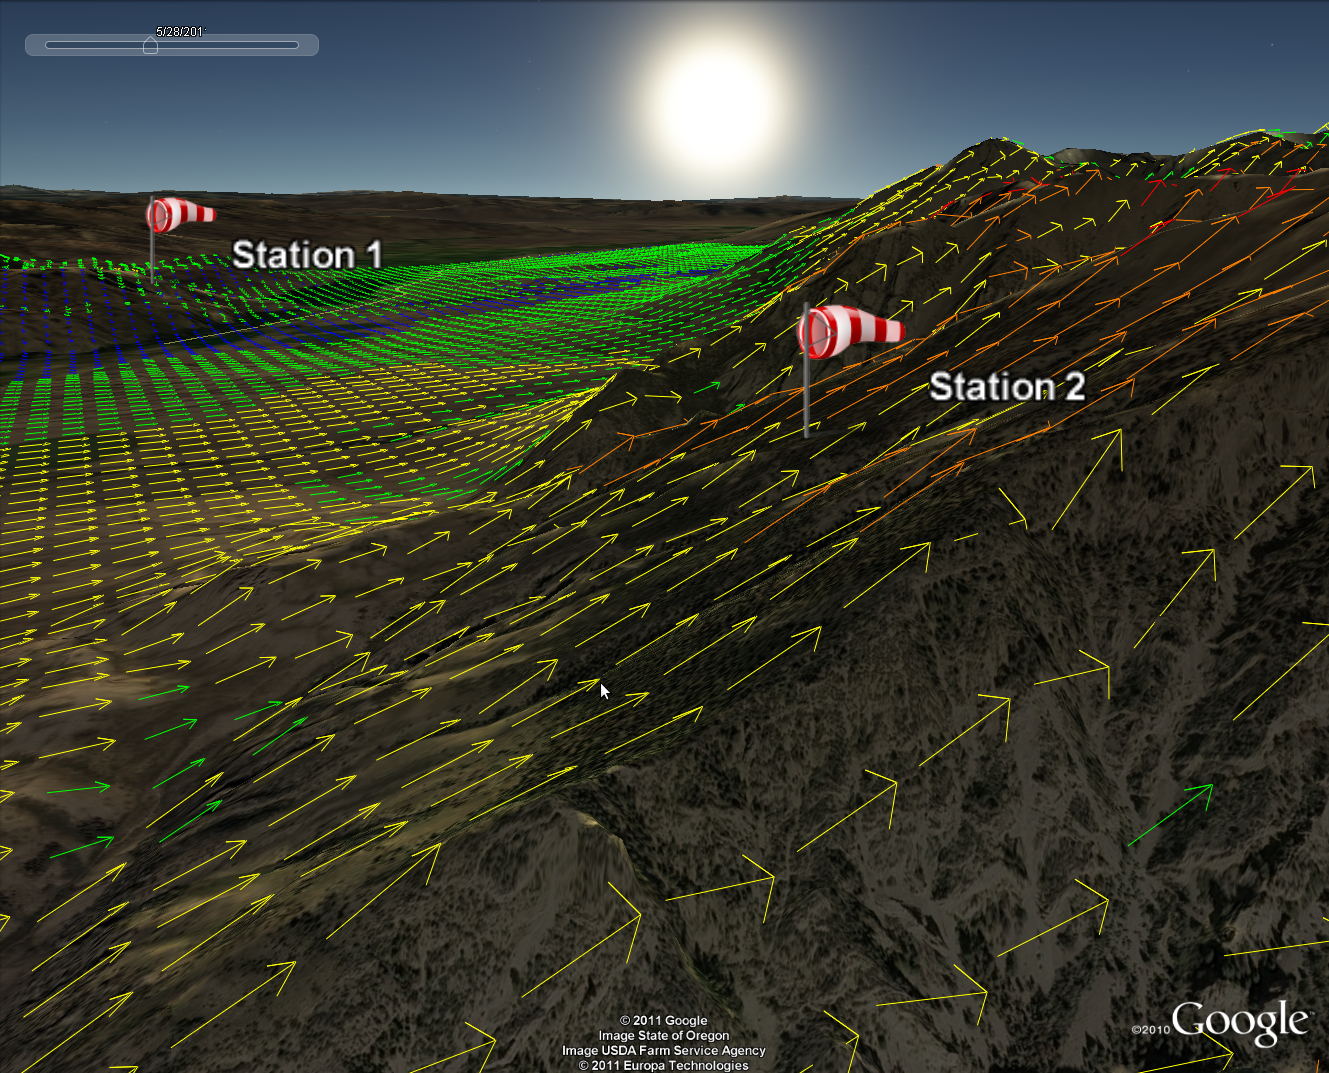
\includegraphics[scale=0.35]							{title_fig}
    \vfill
  	{\Huge
	  3/25/2020 %Date Last Edited
  	}
    \vfill
\end{titlepage}
\section*{Introduction}

Welcome to \textbf{WindNinja Tutorial 3: Point Initialization}.  This tutorial will step you through the process of downloading weather station data and running a WindNinja simulation that is initialized by location specific wind information.  Note that the point initialization option is not currently available for use with the momentum solver. This tutorial assumes you have already gone through \href{https://weather.firelab.org/windninja/tutorials/WindNinja_tutorial1.pdf}{WindNinja Tutorial 1: The Basics} and \href{https://weather.firelab.org/windninja/tutorials/WindNinja_tutorial2.pdf}{WindNinja Tutorial 2: Diurnal Winds and Non-neutral Stability}, and that you have a working Internet connection. After this tutorial, you should feel comfortable using data from weather stations or other observations to initialize your WindNinja runs.

Note:  All required user actions in this tutorial are shown in \textbf{\color{red}red}.

\section*{What is point initialization?}

The point initialization technique in WindNinja allows users to provide input values of wind speed, direction, cloud cover, etc. at specified location(s) on the landscape.  This information is used to drive the simulation, and the final output wind fields will match your inputs at these locations.  Typically, the input information comes from observations at weather stations such as Remote Automated Weather Stations (RAWS) and Automated Airport Weather Stations (ASOS) or from manual measurements done on wildland fires.  But other possibilities exist, and users could even use this method to “craft” their own wind fields.  For readability, this tutorial (and WindNinja) will call these locations “weather stations”, although, as mentioned, they don't necessarily have to be actual weather stations.  You can have as many weather stations as you like, and the stations are not even constrained to be located in the modeling domain. RAWS and ASOS data can be downloaded from MesoWest using a built-in interface.  WindNinja accesses the data through the \href{https://synopticlabs.org/api/mesonet/}{Mesonet API} from Synoptic Labs and the MesoWest Research Group.

\section*{How does point initialization work?}

The first step is to acquire weather station data. Weather station files can be manually constructed (See Section 5), or can be downloaded using the built-in interface. This interface automatically fetches weather data for use in WindNinja simulations. The downloaded data includes all relevant weather data to run a simulation. 

The most recent reported time can be downloaded or a time range can be downloaded.  In the case of a time range, WindNinja must perform time interpolation since each weather station may report weather at a different time.  The user must set the simulation start and stop times and the number of time steps, and WindNinja will interpolate the weather data to these simulation time steps.  WindNinja then runs each step as an individual simulation.

For each simulation, WindNinja reads in all of your weather stations and fills the simulation domain horizontally using an inverse distance interpolation method.  There is a user controlled parameter that allows users to control the radius of influence of each station, if desired.  Then the domain is filled vertically using a vertical wind profile.  Next, diurnal winds are added to this wind field if they are enabled.  Finally, the WindNinja mass-conservation solver is run, including non-neutral stability effects if that option is turned on.  Internally in WindNinja, if this solver was only run once, the resulting wind field would not necessarily match the “measured” wind values at the weather stations anymore (since the winds have been adjusted everywhere to conserve mass).  So instead, WindNinja runs in an iterative way.  After one solver run is finished, WindNinja checks the new wind field to see how close it is to the “measured” values.  If it isn't close enough (less than 0.1 m/s difference), WindNinja slightly adjusts the weather station values and does a new run (i.e., horizontally interpolate, fill vertically, add diurnal, run mass-conservation solver).  This process is repeated until the solved wind field is within 0.1 m/s of the measured values at every weather station.  This is all done automatically by WindNinja, so this process is transparent to the user.  

\section{Getting Started}

\textbf{\color{red}Start WindNinja by going to Start $\Rightarrow$ Programs $\Rightarrow$ WindNinja \vn\ $\Rightarrow$ WindNinja \vn\ }

\section{Input}
\subsection{Surface Input}

\textbf{\color{red}In the navigation tree, left-click on “Surface Input”.}

\textbf{\color{red}
In the input panel, load an elevation file or download one.}

If you are just practicing, you can use an elevation file provided in the WindNinja installation.  They can be found by going to Start WindNinja by going to Start $\Rightarrow$ Programs $\Rightarrow$ WindNinja \vn\ $\Rightarrow$ WindNinja \vn\ $\Rightarrow$Example Files  In the file browser that opens, you will see the elevation file called “missoula\_valley.tif”.

\textbf{\color{red}Select the dominant vegetation type, mesh resolution, and time zone.}

\subsection{Diurnal Input}
Local diurnal slope winds can optionally be included in a point initialization run.  It is normally recommended that diurnal winds be used since it adds more realism to the simulation and increases the simulation time only slightly.

\subsection{Stability Input}

The stability model can optionally be turned on to simulate an atmosphere that is not necessarily neutrally stable.  For this tutorial we will not turn on this model, so leave the “Use Stability” check box unchecked.

\subsection{Wind Input}
\subsubsection{Downloading Weather Stations}

\textbf{\color{red} Left-click on “Point Initialization” in the navigation tree, which is located under “Wind Input”.  In the input panel below, check the “Point Initialization” check box.}

Weather station data can be acquired by opening the station downloader.

\textbf{\color{red}Left-click on “Download data” to open the station downloader window.}

There are two options available for specifying which weather stations to download. The first option is to download all weather stations within the DEM. A buffer can also be set to download stations just outside the DEM. Alternatively, specific weather stations may be downloaded by entering their station IDs by selecting “Download by Station ID”.

Next, you must specify to time period to download data for.  Here you can either download the most recent weather data (one time step), or you can download all available weather data between two date/times.

WindNinja has some limitations to the amount of data that can be downloaded at one time.  This is in place to reduce the load on the server holding the data.  Currently, users are limited to stations within 100 miles of their DEM and up to 1 year of data.  For most users, these limits are not restrictive, but in case they are see Section 6 for details on how to relieve the limits.

The download times are typically very fast, but will depend on the number of stations and time range selected.

\textbf{\color{red}For this tutorial, we will download data using the options “Download from DEM” and “Download Between Two Dates”. Using the Drop-down menu on the right, change the option from “Download Most Recent Data” to Download Between Two Dates”. Your screen should look similar to this:}

\begin{figure}[H]
	\centering
	\label{}
	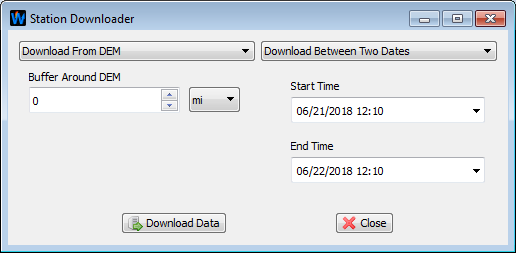
\includegraphics[scale=1.0]{SF-1-2}
\end{figure}

The start and stop time may be edited to change the range over which data is downloaded. The default is to download data from right now to 24 hours ago at this time.  For this tutorial, we will use the defaults.

\textbf{\color{red}Click “Download Data” to download the station data. A pop-up progress bar will display the status of the download. When this is complete, click “close” and exit the Station Downloader.}

\begin{figure}[H]
	\centering
	\label{}
	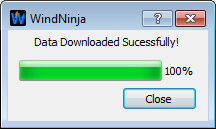
\includegraphics[scale=1.0]{Download-3}
\end{figure}

\subsection{Selecting Weather Stations}
Once your download is finished and you exit the station downloader, a new folder beginning with “WXSTATIONS”, will appear in the main panel under “Select Weather Stations”. All of your downloaded weather stations will appear in this panel. You can download multiple weather stations and they will be added to this list.  This weather stations panel is an expandable tree structure showing the files and folders that are valid for point initialization runs. You can expand these folders to select the .csv weather station files. Note that all times in the point initialization tab are based on the surface input time zone unless otherwise specified.

If you generate your own weather station files, or acquire them from other sources, these can also be selected. To use these files, place them in the same directory as your DEM and WindNinja will automatically detect, and make them selectable in the weather stations panel.

The folder name containing the downloaded weather stations follows a specific format. For example:

\begin{figure}[H]
	\centering
	\label{}
	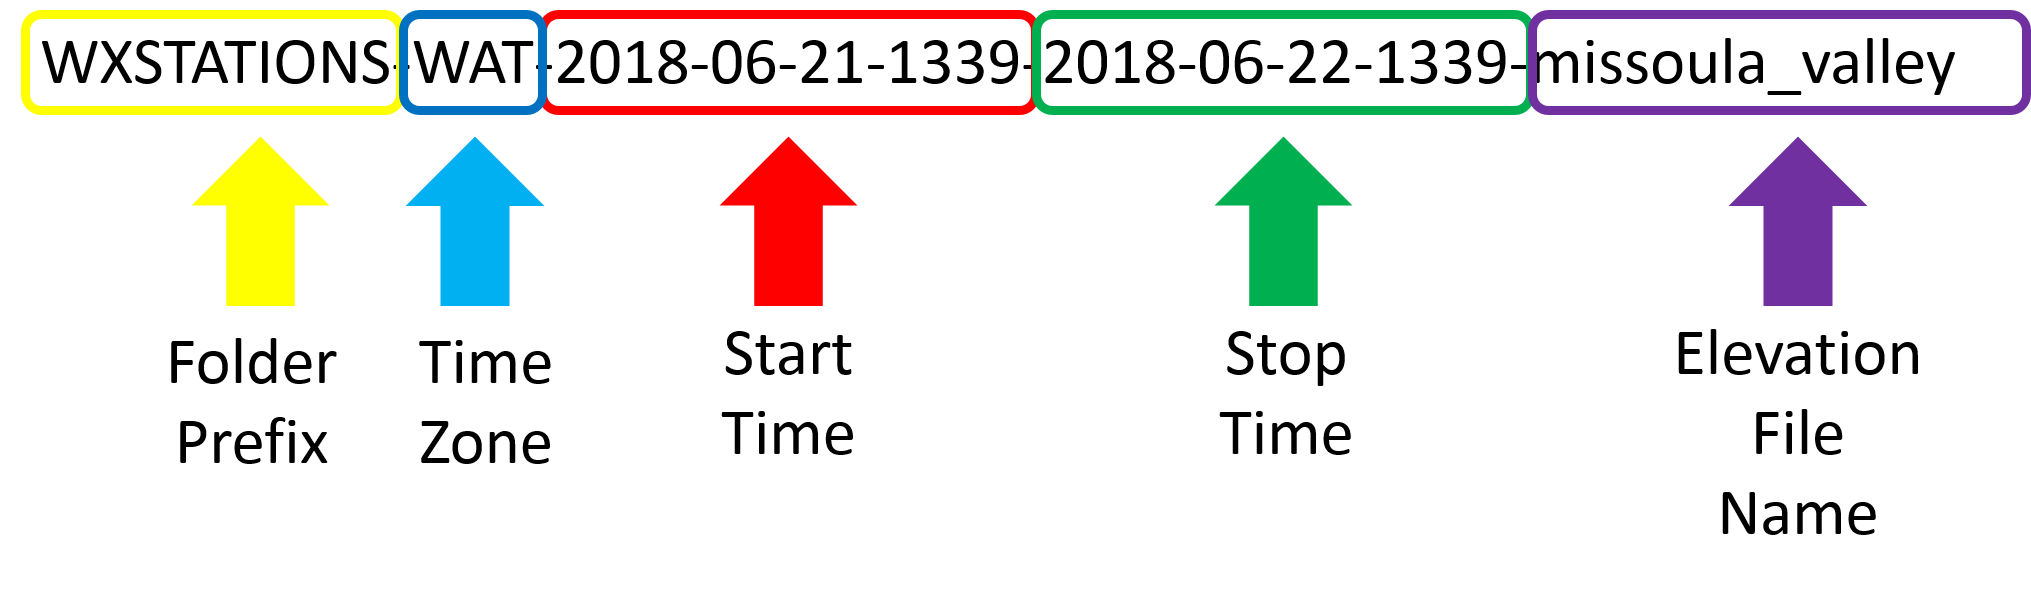
\includegraphics[scale=0.45]{FolderDiag_1}
\end{figure}

All of the weather station files are stored in this folder. Each file inside the folder is a unique weather station, and naming follows a similar naming format. For example:

\begin{figure}[H]
	\centering
	\label{}
	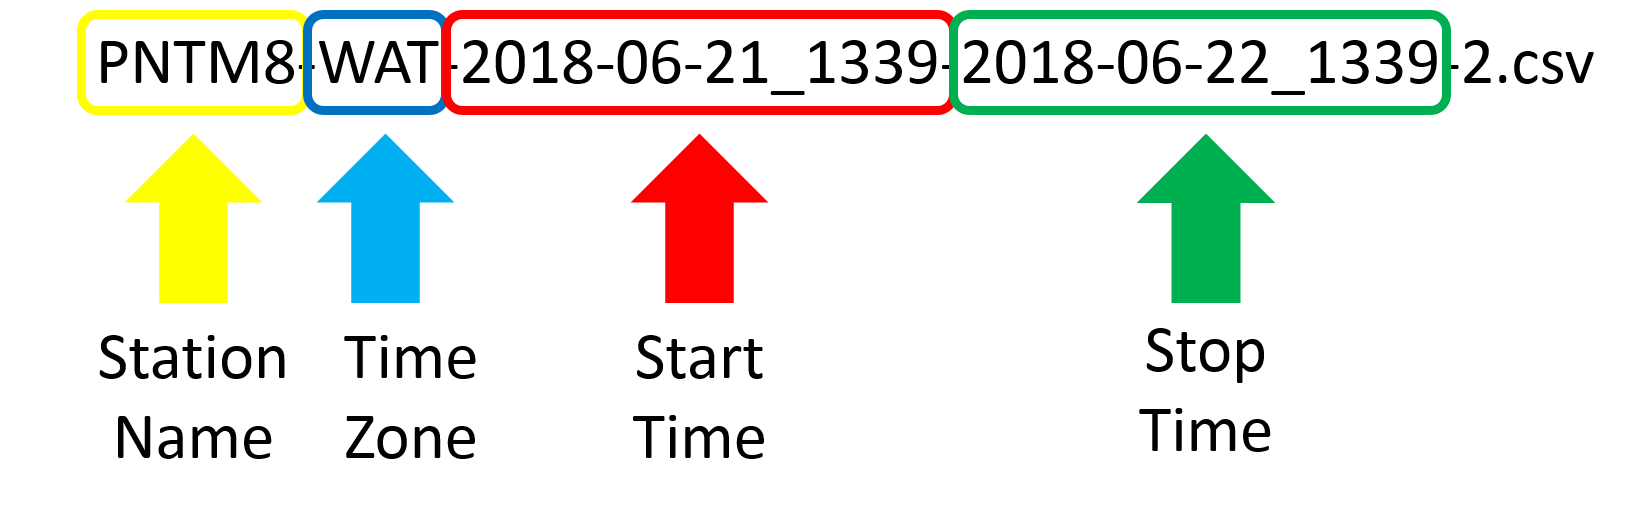
\includegraphics[scale=0.45]{FileDiag_1}
\end{figure}

\textbf{\color{red}Select the desired weather stations by left clicking \underline{each} file you want to use.}

\begin{figure}[H]
	\centering
	\label{}
	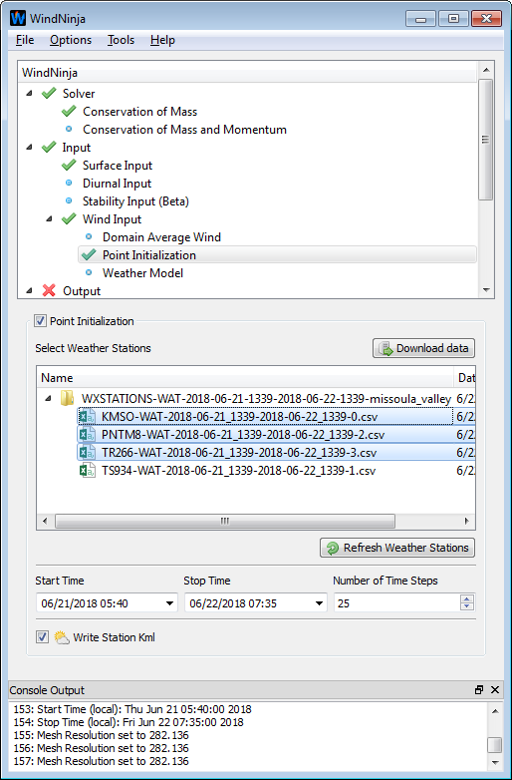
\includegraphics[scale=1.0]{PI-Select-Blue_1}
\end{figure}

Note that there are several different types of weather station file formats that are valid  for point initialization runs, however they are incompatible with each other.

\subsubsection{Types of Weather Stations}
\begin{enumerate}
	\item  \underline{Time series}: Each file is a unique weather station and these files have multiple observations per station. You can select as many time series files as long as at least some of the data overlaps with the selected simulation start and stop times. This format is the only type that supports multiple time step runs.
	\item \underline{Single Step}: Each file is a unique weather station, and these files have only one time-naive observation. These files are produced by selecting the “Download Most Recent Data” option. You can select as many Single Step  files as you want. These files may not be used for multiple time step runs.
	\item \underline{Old Station Format}: All weather stations are contained in one file, and only work for a single time step. These files are incompatible with all other file formats, and only one file may be selected. This format is not recommended and supported only for legacy users.  
\end{enumerate}

After you select the files you would like to use, the start and stop time for the simulation are automatically populated based on the start and stop times that the weather stations have on disk. The simulation times can be manually changed by editing the start and stop time. The “Number of Time Steps” box allows you to change how many simulations you want to run between the start and stop time. These time steps are evenly spaced between the start and stop time.  WindNinja will automatically suggest a number of time steps based on the number of hours between the start and stop start and stop times.  For this tutorial, we will use the defaults.

Note that if you choose \underline{Single Step}files, the simulation time is fixed to when the file was downloaded. \underline{Old Station Format} files require date and time input from the user.

For your convenience, there is a button at the bottom of the input panel called “Write Station KML” that will write a Google Earth file showing the locations of the weather stations and their values.

\textbf{\color{red} Click “Write Station KML” to write a .kml of the weather stations for viewing in Google Earth. One .kml will be written per time step.}

\section{Output}

The same output files are written for point initialized simulations as for other simulations. WindNinja does a separate simulation for each time step and writes separate output files for each of these steps.

\textbf{\color{red} In the navigation tree, left-click on “Output” and select the “Output Height”, “Output Speed Units”, and  “Clip output by:” values you desire.}

\textbf{\color{red} Choose the types of output files you would like by left-clicking the type in the navigation tree and filling out the corresponding input panel.}

If you enable the Fire Behavior output files, note that the percent cloud cover file that is produced during a point initialized run is a gridded file that uses inverse distance squared weighted interpolation to fill the grid based on the input values at the weather stations.

\section{Solve}

\textbf{\color{red}Left-click on “Solve” in the navigation tree.  Set the number of processors you would like using the “Number of Processors” spin box.  Finally, left-click the “Solve” button to start the simulation.}

The typical simulation time for an average dual core computer in 2011 should be around 10-60 seconds depending on the computer, domain size, simulation resolution, number of steps, etc.

\textbf{\color{red} When the simulation is finished, close the progress window.}

\textbf{\color{red}Another handy feature in WindNinja is the “Open Output Files Path” button on the Solve page.  If you click this, it will open the folder where all of the output files for the last run were written to.}

\section{Building Your Own Station Files}\label{growyourown}

Instead of downloading station files, you can make your own if you have weather information from some other source.  A blank station file can be generated by selecting \textit{Tools} $\Rightarrow$ \textit{Write Blank Station File}. Each file corresponds to a single weather station and each line in the file corresponds to an observation.

The example station file viewed in a spreadsheet program is shown in Table 1 below.

Note that the station file could also be opened and edited in a simple text editor such as WordPad or NotePad, but it is more convenient and less error prone in a spreadsheet program.  Also be aware that in a text editor it doesn't look exactly like Table 1, instead there will be commas separating each field.

Several sample weather stations have been included with your installation. In the WindNinja example files, locate folders called WXSTATIONS-2018-06-25-1237-missoula\_valley (a single step set of weather stations) and WXSTATIONS-MDT-2018-06-20-2128-2018-06-21-2128-missoula\_valley (a time series set of weather stations). The format of each of these files looks similar to the example file below.

\begin{landscape}
\begin{figure}[H]
	\centering
	\label{}
	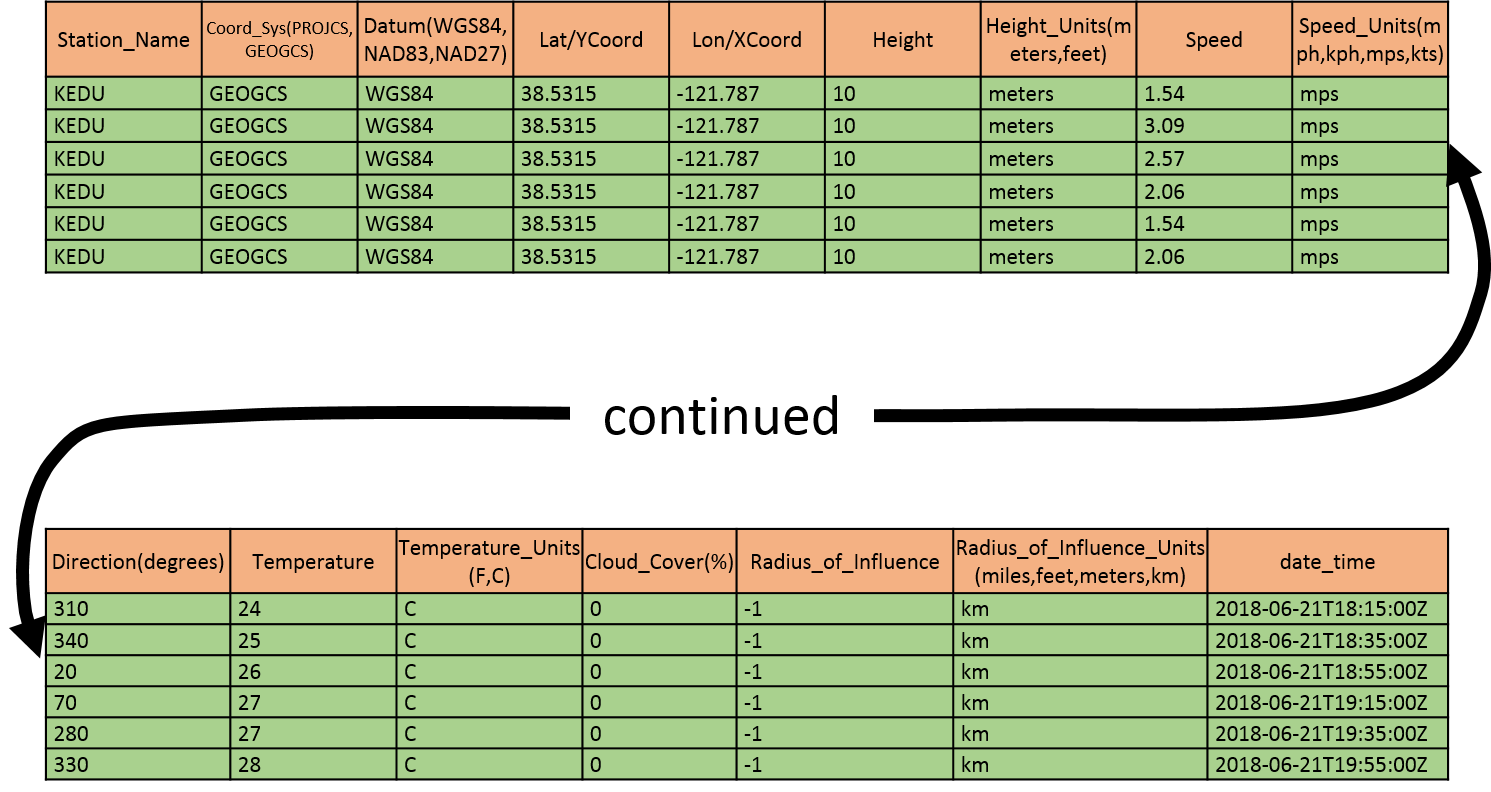
\includegraphics[scale=0.9]{Table-1}
\end{figure}
\end{landscape}
The format of a station file is that the first row is a header that tells you what goes in the corresponding columns.  The header fields may contain a textual description of the column, units information, and/or a list of valid values.  Every row below the header row represents a measurement for the weather station (ie. each row is a different date/time).  A short description of each column is given below.

\textbf{Station\_Name}

This is the name of the weather station. Stations downloaded through WindNinja use their Station ID, for example “Point 6 RAWS” is stored as “PNTM8”.

\textbf{Coord\_Sys}

This is the coordinate system that you will be specifying the location of the station in (later).  The two possible choices are “PROJCS” and “GEOGCS”.  PROJCS stands for “projected coordinate system”.  If you use this, you will specify the location of the station in x,y coordinates in meters.  The projection you are actually using is the one that the elevation file is in (for example, UTM, Albers, etc.).  This might be useful if you are viewing your elevation file and locating the weather stations in a GIS, since the GIS probably outputs locations in the elevation file's projected coordinate system.  The other choice, GEOGCS, stands for “geographic coordinate system” or, in other words, latitude and longitude.  So if you want to specify the location of the station in latitude and longitude, use GEOGCS.  This would be useful if you knew the latitude/longitude of the weather station or had coordinates from a GPS or were using something like Google Earth to determine where the station will be (since the default in Google Earth is to output position in latitude/longitude). Stations downloaded through WindNinja use GEOGCS.

\textbf{Datum}

This is the datum that will be used for specifying the location of your weather station.  The possible choices are “WGS84”, “NAD83”, or “NAD27”.  Note that if you specified PROJCS in the last column for \textbf{Coord\_Sys}, then the datum defined by the elevation file will also be used automatically by WindNinja, so in that case it doesn't matter what you choose (but you need to put something here as a place holder).  Also note that if you are using Google Earth to obtain the lat/long of a weather station, Google Earth uses “WGS84”.

\textbf{Lat/YCoord}

This is either the latitude or y-coordinate of the weather station, depending on your choice for the \textbf{Coord\_Sys} earlier.

\textbf{Lon/XCoord}

This is either the longitude or x-coordinate of the weather station, depending on your choice for the \textbf{Coord\_Sys} earlier.

\textbf{Height}

This is the height of the measured wind above the surrounding vegetation (measured as the distance above the vegetation, not necessarily above the ground).  Typically this might be 20 feet or 10 meters. Airport (ASOS) stations measure wind speed at 10 m (~32ft) , permanent RAWS typically report wind speed at 20 ft (~6 m), and Incident RAWS (IRAWS) typically report wind speed at 6 ft (~2 m).

\textbf{Height\_Units}

The units your height is measured in.  Valid choices are “meters” or “feet”.

\textbf{Speed}

This is the wind speed at the weather station.

\textbf{Speed\_Units}

The units of the wind speed.  Valid choices are “mph”, “kph”, “m/s”, and “kts”.

\textbf{Direction}

This is the wind direction, using the normal meteorologic convention that it is the direction that the wind \textit{comes from}.  So for example, if the wind was blowing from west to east, it would be a direction of 270.

\textbf{Temperature}

Air temperature at the station.  This is used in the diurnal submodel.  It should be noted that the simulated wind is not very sensitive to this value and anything close should be adequate.

\textbf{Temperature\_Units}

The units of temperature.  Valid choices are “F” or “C”.

\textbf{Cloud\_Cover}

The percent cloud cover (not fractional cloud cover).  The valid range is 0-100.  This is used in the diurnal and non-neutral stability submodels.

\textbf{Radius\_of\_Influence}

This is an option that allows you to limit the horizontal distance that the weather station can affect.  If you specify a distance less than zero, this is a special flag that tells WindNinja that this station has no imposed distance limit.  Your default should be to enter a value less than zero (like “-1”) to use no distance limit for most stations.  An actual distance limit could be used if you think your weather station is being influenced by local factors and doesn't represent the larger scale wind well.  This might be the case if the station was located in the lee wind area of a mountain where the measured wind was affected by the mountain's wake.  Note that you must have at least one weather station without a distance limit (value less than zero) so that the whole simulation domain will be filled with initial wind values.

\textbf{Radius\_of\_Influence\_Units}

The distance units of the radius of influence.  Valid choices are “feet”, “miles”, “meters”, and “km”.

\textbf{date\_time}

The observation date and time stored in UTC. Format:  \texttt{YYYY-MM-DDTHH:MM:00Z}. Seconds are not supported at this time. If this is left blank, only one observation may be stored in the file, and it may not be used for multiple time step runs.

\section{Using a Custom API token}

If you want to download more data than WindNinja  allows (1 year and stations within a 100 mile buffer from your DEM), you will need to specify your own \textbf{token} for the Mesonet API (this is related to the code WindNinja uses to download weather data from MesoWest). To do this, follow the instructions on \url{https://synopticlabs.org/api/mesonet/} to get an API key and \textbf{token}.

Once you have a \textbf{token}, you can specify in WindNinja via the configuration option \texttt{CUSTOM\_API\_KEY}.

In the graphical user interface this is accomplished by going to Tools $\Rightarrow$ Configuration Option. In option field, type: \texttt{CUSTOM\_API\_KEY}, and insert your \textbf{token} in value field.  Click OK, to finalize.

\begin{figure}[H]
	\centering
	\label{}
	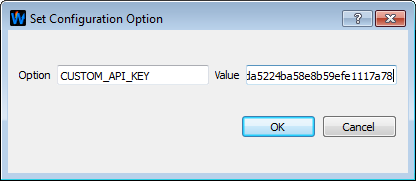
\includegraphics[scale=1]{api-config}
\end{figure}

This concludes \textbf{Windinja Tutorial 3: Point Initialization}

\section*{Acknowledgements}
The incorporation of weather station downloads in WindNinja was made possible in part due to the data made available by \href{https://synopticlabs.org/api/mesonet/}{MesoWest/SynopticLabs} though the Mesonet API.


\end{document}